\documentclass[main.tex]{subfiles}

\section{Design your own Explicit Runge-Kutta Method}
\subsection{Order conditions, coefficients for the error estimator and the Butcher tableau}
Using the excerpt from the book provided in the lecture 10 folder we will write up the order conditions for an embedded Runge-Kutta method with
3 stages. The solution will have order 3 and the embedded method used for error estimation will have order 2.

Firstly the Butcher tableau for our ERK will have the following schema (henceforth the upper triangular shape where the $a_{ij}$ coefficients are $0$ and $c_1 = 0$):
\begin{table}[h]
    \centering
    \begin{tabular}{l | c c c }
        0 & 0 & 0 & 0 \\
        $c_2$ & $a_{21}$ & 0 & 0 \\
        $c_3$ & $a_{31}$ & $a_{32}$ & 0 \\
        \hline
        $x$ & $b_1$ & $b_2$ & $b_3$ \\
        $\widehat{x}$ & $\widehat{b}_1$ & $\widehat{b}_2$ & $\widehat{b}_3$ \\
        \hline
        $e$ & $d_1$ & $d_2$ & $d_3$
    \end{tabular}
    \caption{Butcher tableau for ERK with 3 stages and embedded method}
\end{table}
\begin{subequations}
\\Order conditions (one for first order, one for second order and two for third order) derived from our Butcher tableau:
\begin{align}
    &\mathcal{O}(h^1):& b^T e &= 1 & &b_1 + b_2 + b_3 = 1 & \tau_1 &\rightarrow \rootedtree[] \\
    &\mathcal{O}(h^2):& b^T C e &= \frac{1}{2} & &\underbrace{b_1 c_1}_{0} + b_2 c_2 + b_3 c_3 = \frac{1}{2} & \tau_2 &\rightarrow \rootedtree[*] \\
    &\mathcal{O}(h^3):& b^T C^2 e &= \frac{1}{3} & &\underbrace{b_1 c_1^2}_{0} + b_2 c_2^2 + b_3 c_3^2 = \frac{1}{3} & \tau_3 &\rightarrow \rootedtree[*,*] \\
    & & b^T A C e &= \frac{1}{6} & &\underbrace{b_2 a_{21} c_1}_{0} + \underbrace{b_3 a_{31} c_1}_{0} + b_3 a_{32} c_2 = \frac{1}{6} & \tau_4 &\rightarrow \rootedtree[[*]]
\end{align}
values of $c_2$ and $c_3$ will be set to $\frac{1}{4}$ and $1$ respecively. This leaves us with 6 unknown variables (3 $a$s and 3 $b$s) and only 4 equations so we will add the so called consistency conditions in order for the system to be solvable.
\begin{align}
    c_2 &= a_{21} \\
    c_3 &= a_{31} + a_{32}
\end{align}
\end{subequations}
Using Matlab to solve the system we get the following results: 
\begin{center}
    $b_1 = -\frac{1}{6}$, $b_2 = \frac{8}{9}$, $b_3 = \frac{5}{18}$, $a_{21} = \frac{1}{4}$, $a_{31} = -\frac{7}{5}$, $a_{32} = \frac{12}{5}$.
\end{center}

Next we will solve the system defined for second order embedded method with one first order and one second order condition where $c_2$ and $c_3$ are known thus giving 2 equations with 3 unknowns. In order to find a solution, $\widehat{b}_2$ is set to be $\frac{1}{2}$\footnote{According to the book excerpt given in Lecture 10 folder. Otherwise any real value < 1 could have been selected.}.
\begin{subequations}
\begin{align}
    \widehat{b}_1 + \widehat{b}_2 + \widehat{b}_3 &= 1 \\
    \widehat{b}_2 c_2 + \widehat{b}_3 c_3 &= \frac{1}{2}
\end{align}
\end{subequations}
The above system yields $\widehat{b}_1 = \frac{1}{8}$ and $\widehat{b}_3 = \frac{3}{8}$. Going back to the Butcher tableau we know that last row $e = (d_1, d_2, d_3)$ is just the difference of the previous two rows by definition.

\begin{table}[h]
    \centering
    \begin{tabular}{r | C C C }
        $c_1 = 0$ & 0 & 0 & 0 \\
        $c_2 = \frac{1}{4}$ & 1/4 & 0 & 0 \\
        $c_3 = 1$ & -7/5 & 12/5 & 0 \\
        \hline
        $x$ & -1/6 & 8/9 & 5/18 \\
        $\widehat{x}$ & 1/8 & 1/2 & 3/8 \\
        \hline
        $e$ & -7/24 & 7/18 & -7/72
    \end{tabular}
    \caption{Butcher tableau with error estimators for our method}
    \label{tbl:our-butcher}
\end{table}

% Test equation
\subsection{Testing on the test equation}
Figure \ref{fig:ex3testeq} depicts designed method and the analytical solution for various step sizes ($0.1$, $0.01$, $0.001$) in the rows along with absolute error (difference between true value of the test equation and the result of the designed method), the maximum error is shown in the plot's title as well as in a reference line. From the previously mentioned figure it is clear that the designed method works as expected.
\begin{figure}[H]
    \centering
    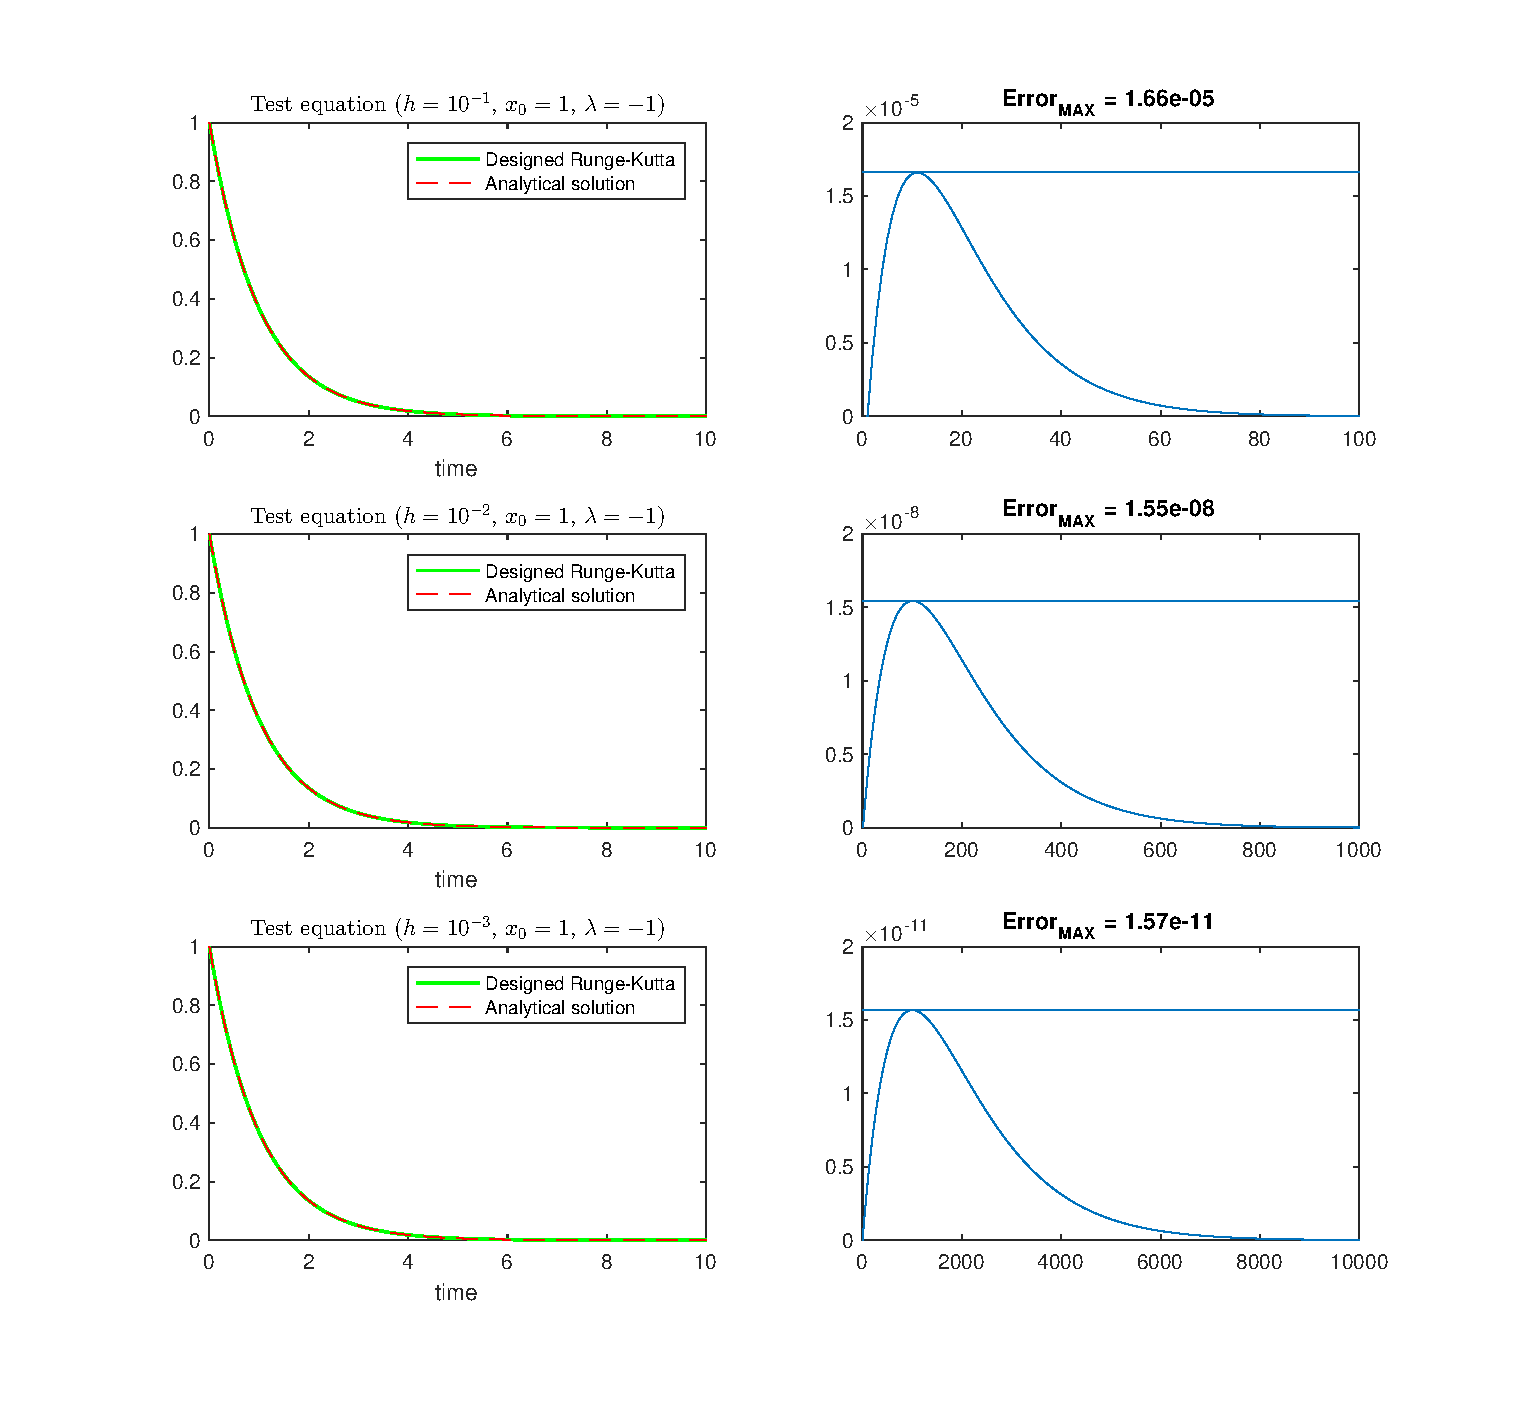
\includegraphics[width=\textwidth]{../Figures/ex3_testequation}
    \caption{Comparison with the test equation for different step sizes}
    \label{fig:ex3testeq}
\end{figure}

% Verify the order
\subsection{Verifying the order}
Ten step sizes between $10^{-3}$ and $10^{-1}$ spaced logarithmicaly were chosen to plot the local error as a function of the step size. Loglog plot \ref{fig:ex3loglog} along with dashed help lines is used in order to verify the order of the method designed. It can be seen that both entries are parallel with the help lines for $\mathcal{O}(h^3)$ and $\mathcal{O}(h^2)$ respectively, confirming that the method designed meets the order criteria specified in the beginning of this section.
\begin{figure}[H]
    \centering
    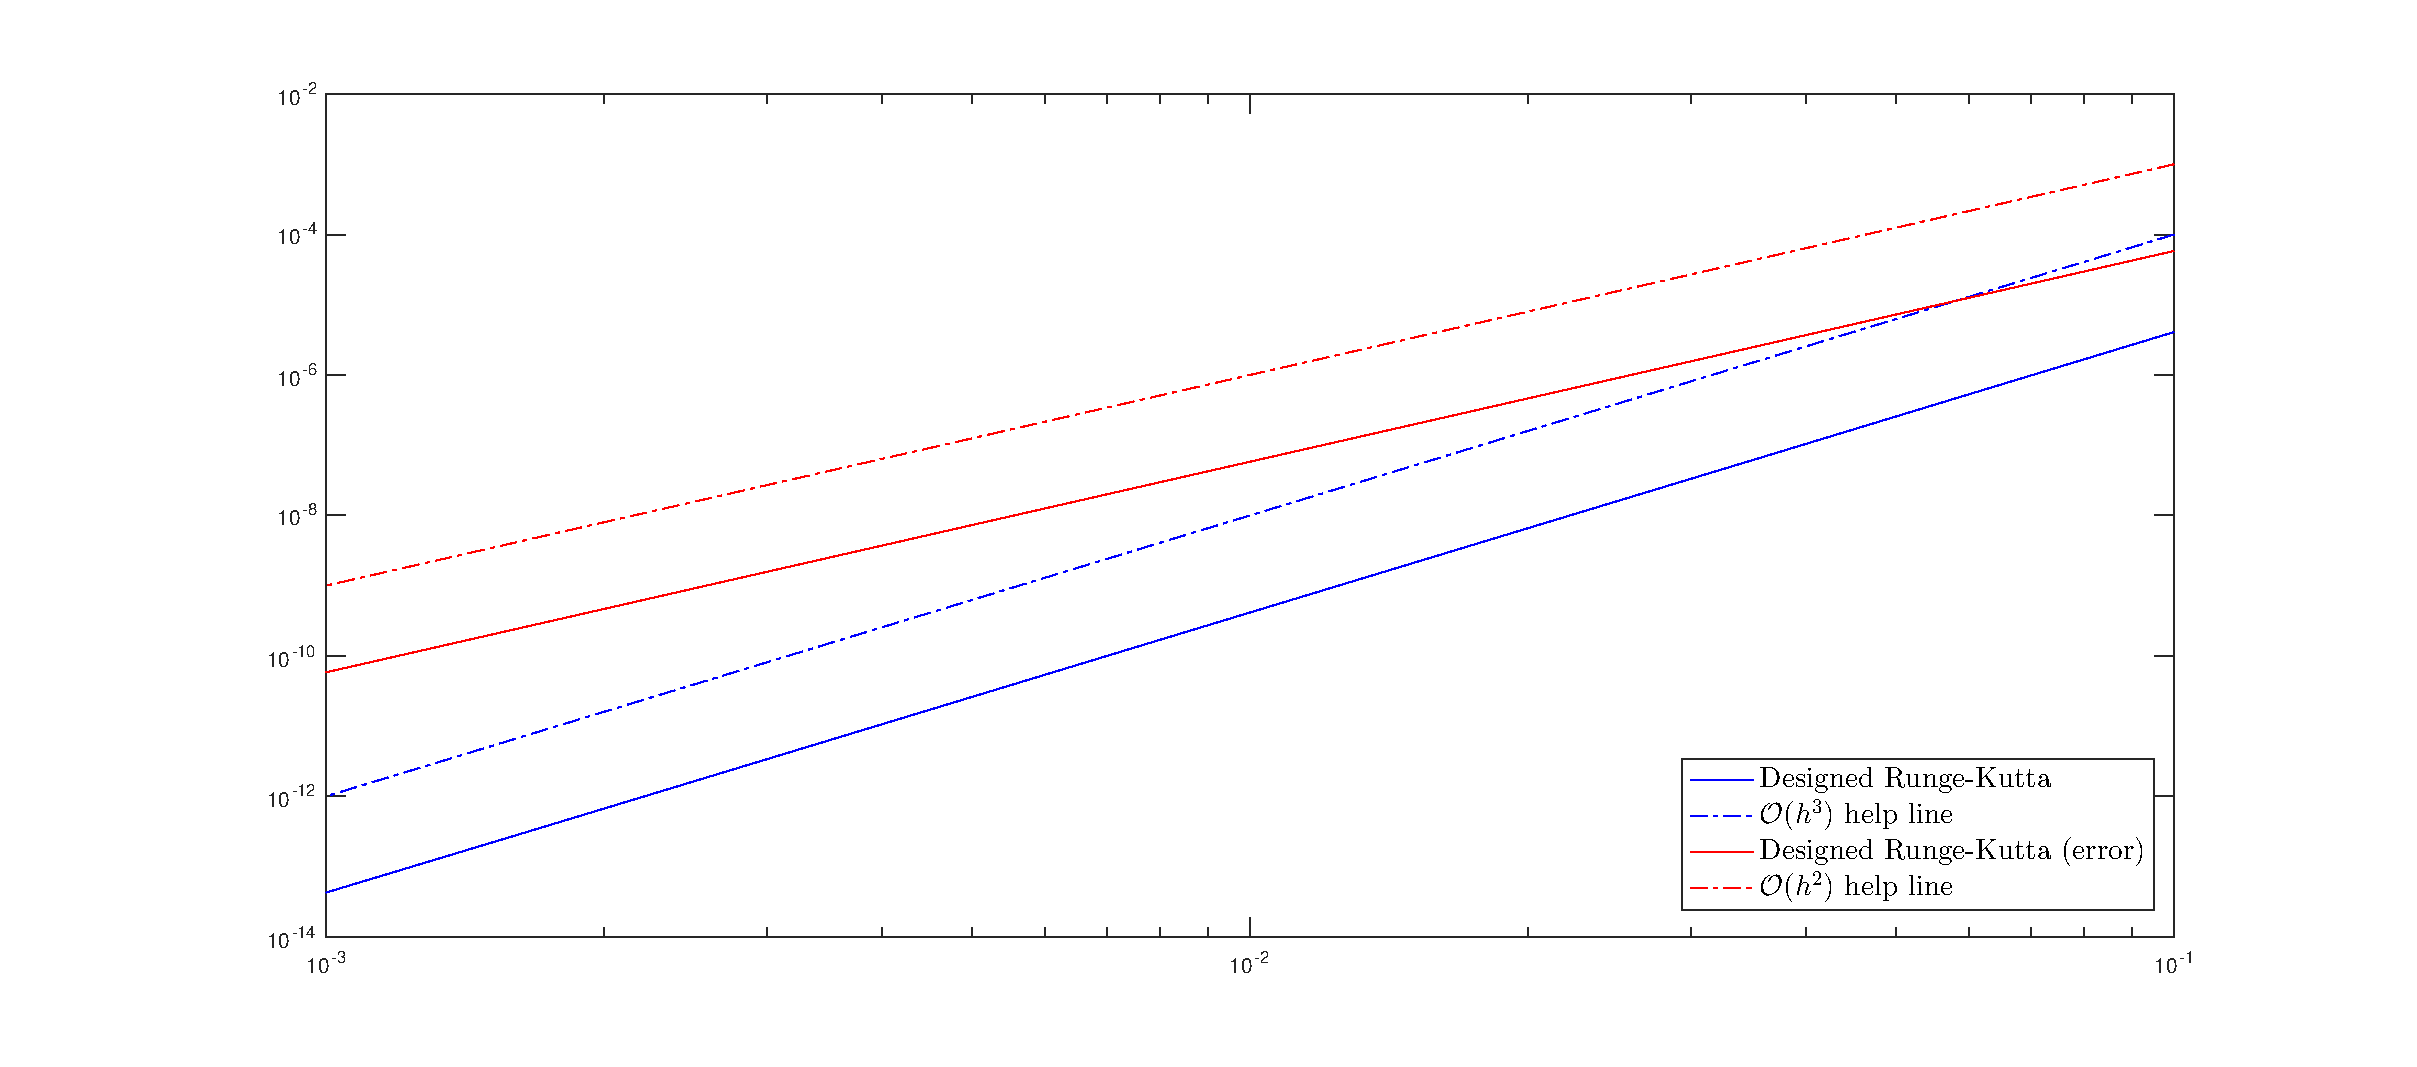
\includegraphics[width=\textwidth]{../Figures/ex3_ERK23localerror}
    \caption{Loglog plot of the local error of designed ERK method (blue) and the returned error of the method (red, local error estimate) with help lines}
    \label{fig:ex3loglog}
\end{figure}

% Computing R(z) and stability plots
\subsection{$\mathbf{R(\lambda h)}$ and stability plot}
The solution to the test equation obtained by a Runge-Kutta method is defined as $x(t_n + h) = R(\lambda h) x(t_n)$ and $R(z) = 1 + z b^T ({I} - z {A})^{-1} e$. From the \nameref{tbl:our-butcher} vector $b$ and the $A$ matrix are plugged in to $R(z)$ resulting in \[R_m(z) = 1 + z + \frac{1}{2} z^2 + \frac{3}{18}z^3\] where $z = \lambda h$ for the third order method.
The second order embedded method yields \[R_e(z) = z+ \frac{1}{2} z^2 + \frac{9}{40} z^3\] where $z = \lambda h$. Note that $R(z)$ can be calculated with Matlab's Symbolic Toolbox \\\texttt{syms z};\\ \texttt{R = 1 + z*b'*inv(eye(length(b)) - z*A)*ones(length(b),1)};\\ then \texttt{collect(R, z)} is used display powers of $z$ and the respective coefficients.

The difference in stability of the designed and embedded method can be seen in figure \ref{fig:ex3stab}. Although the plots look similar, the embedded method's stability region is slightly smaller, as well as all other metrics.

\begin{figure}[H]
    \centering
    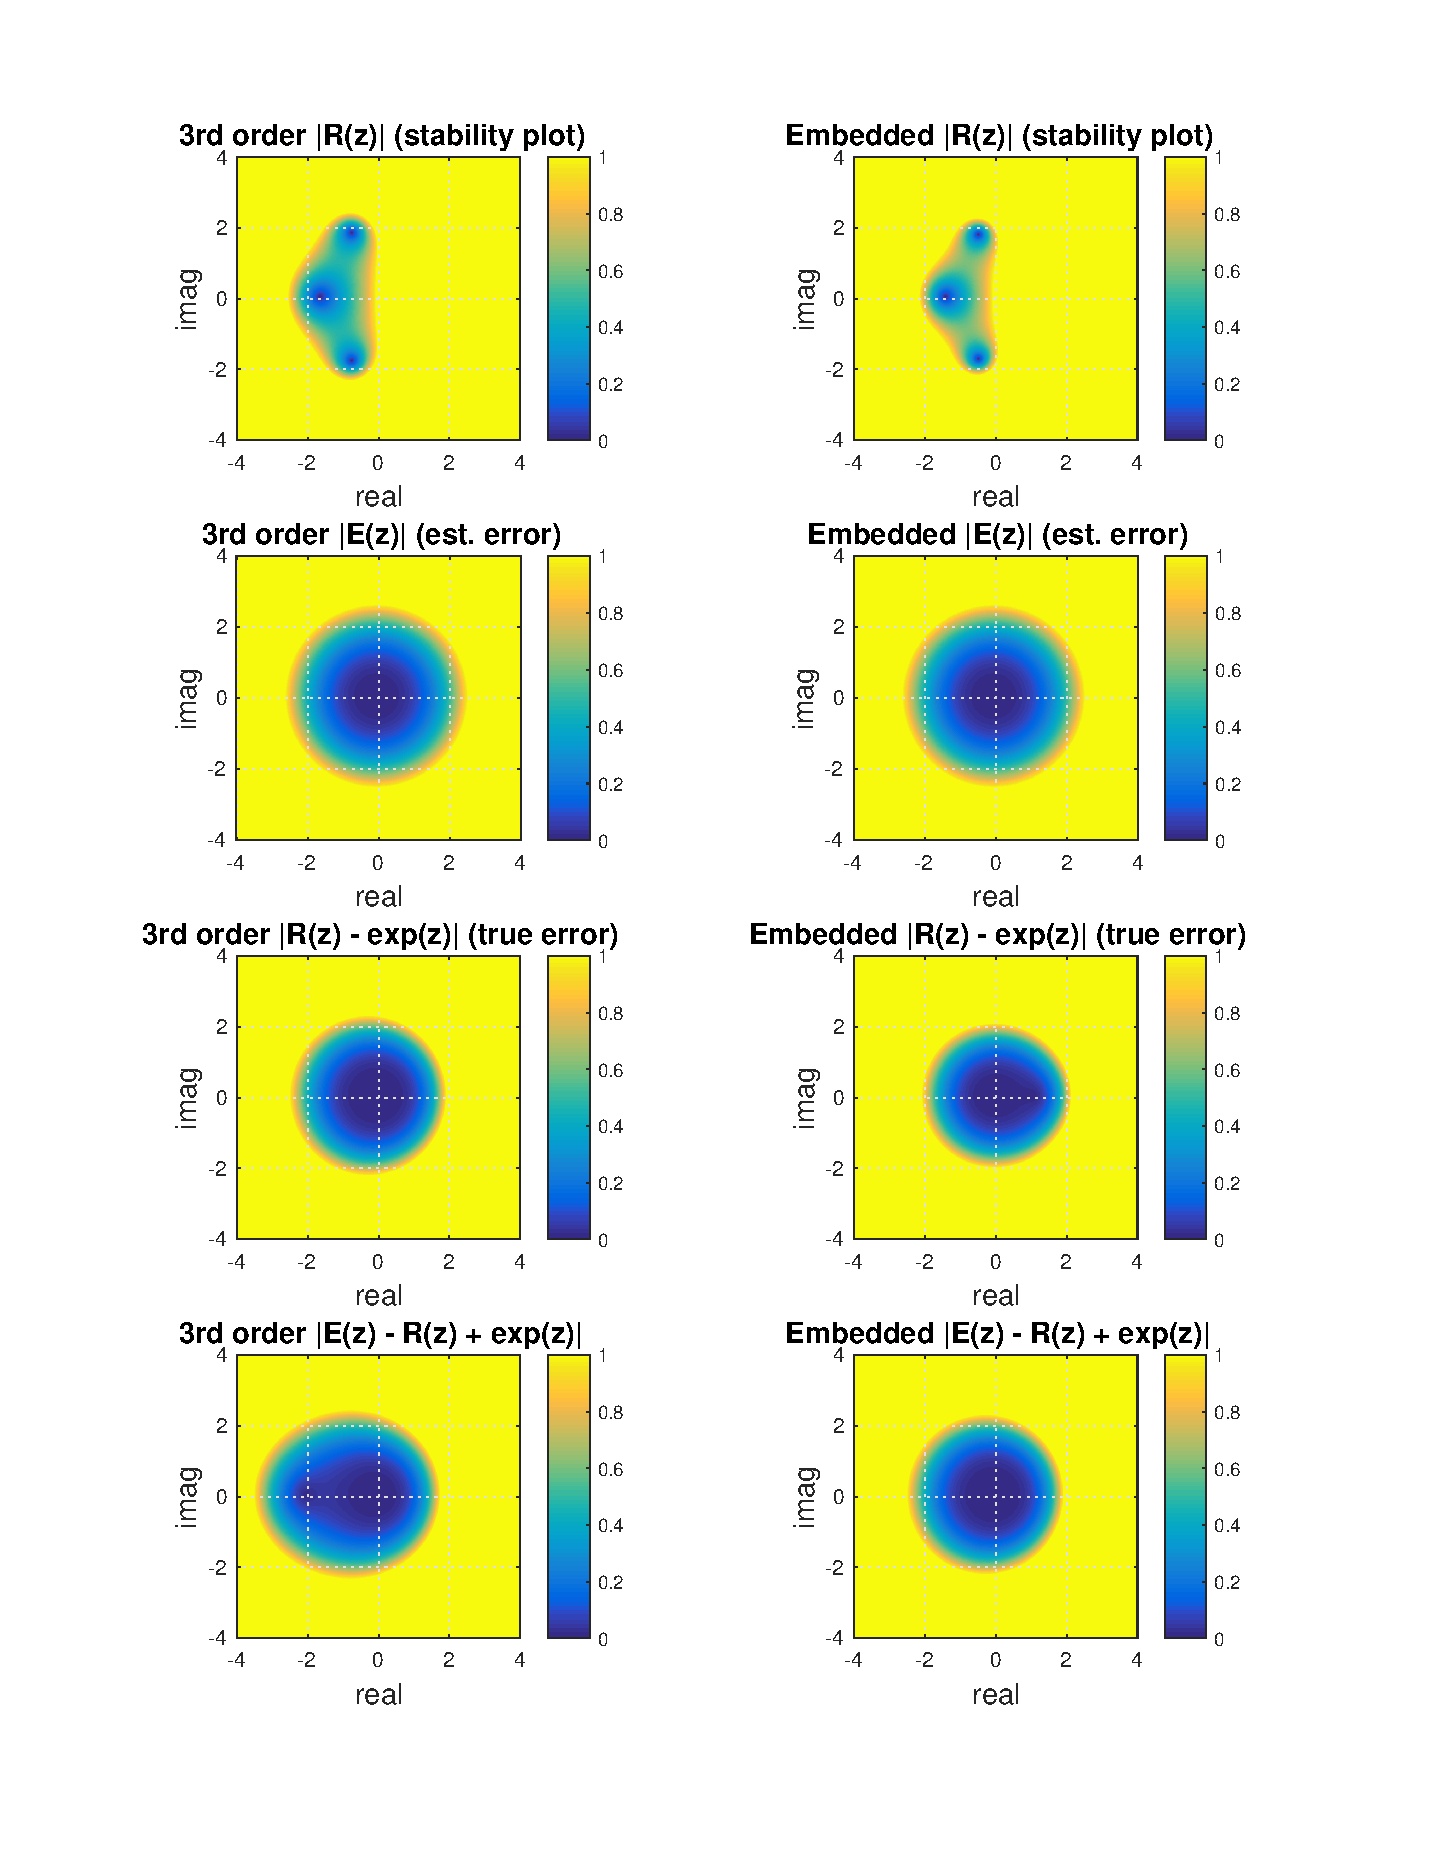
\includegraphics[width=\textwidth,trim={0 0.5cm 0 0.5cm},clip]{../Figures/ex3_stabilityplot}
    \caption{Stability plots of the third order ERK with second order embedded method. In order for the method to be A stable the whole left half plane has to be $|R(z)|<1$ (i.e. in graphical representation shown not brightly yellow) which clearly it is not.}
    \label{fig:ex3stab}
\end{figure}

% Van der pol and ode15s
\subsection{Testinging on the Van der Pol problem and comparison with \texttt{ode15s}}
Matlab's \texttt{ode15s} was used with the default ODE-options and user defined Jacobian, the error for our method with with step size of $10^{-3}$ is roughly around $10^{-8}$ and for step size $10^{-2}$ it is around $10^{-5}$. Even though our choice of $c_2 = 1/4$ might look strange, the method performs reasonably well.

\begin{figure}[H]
    \centering
    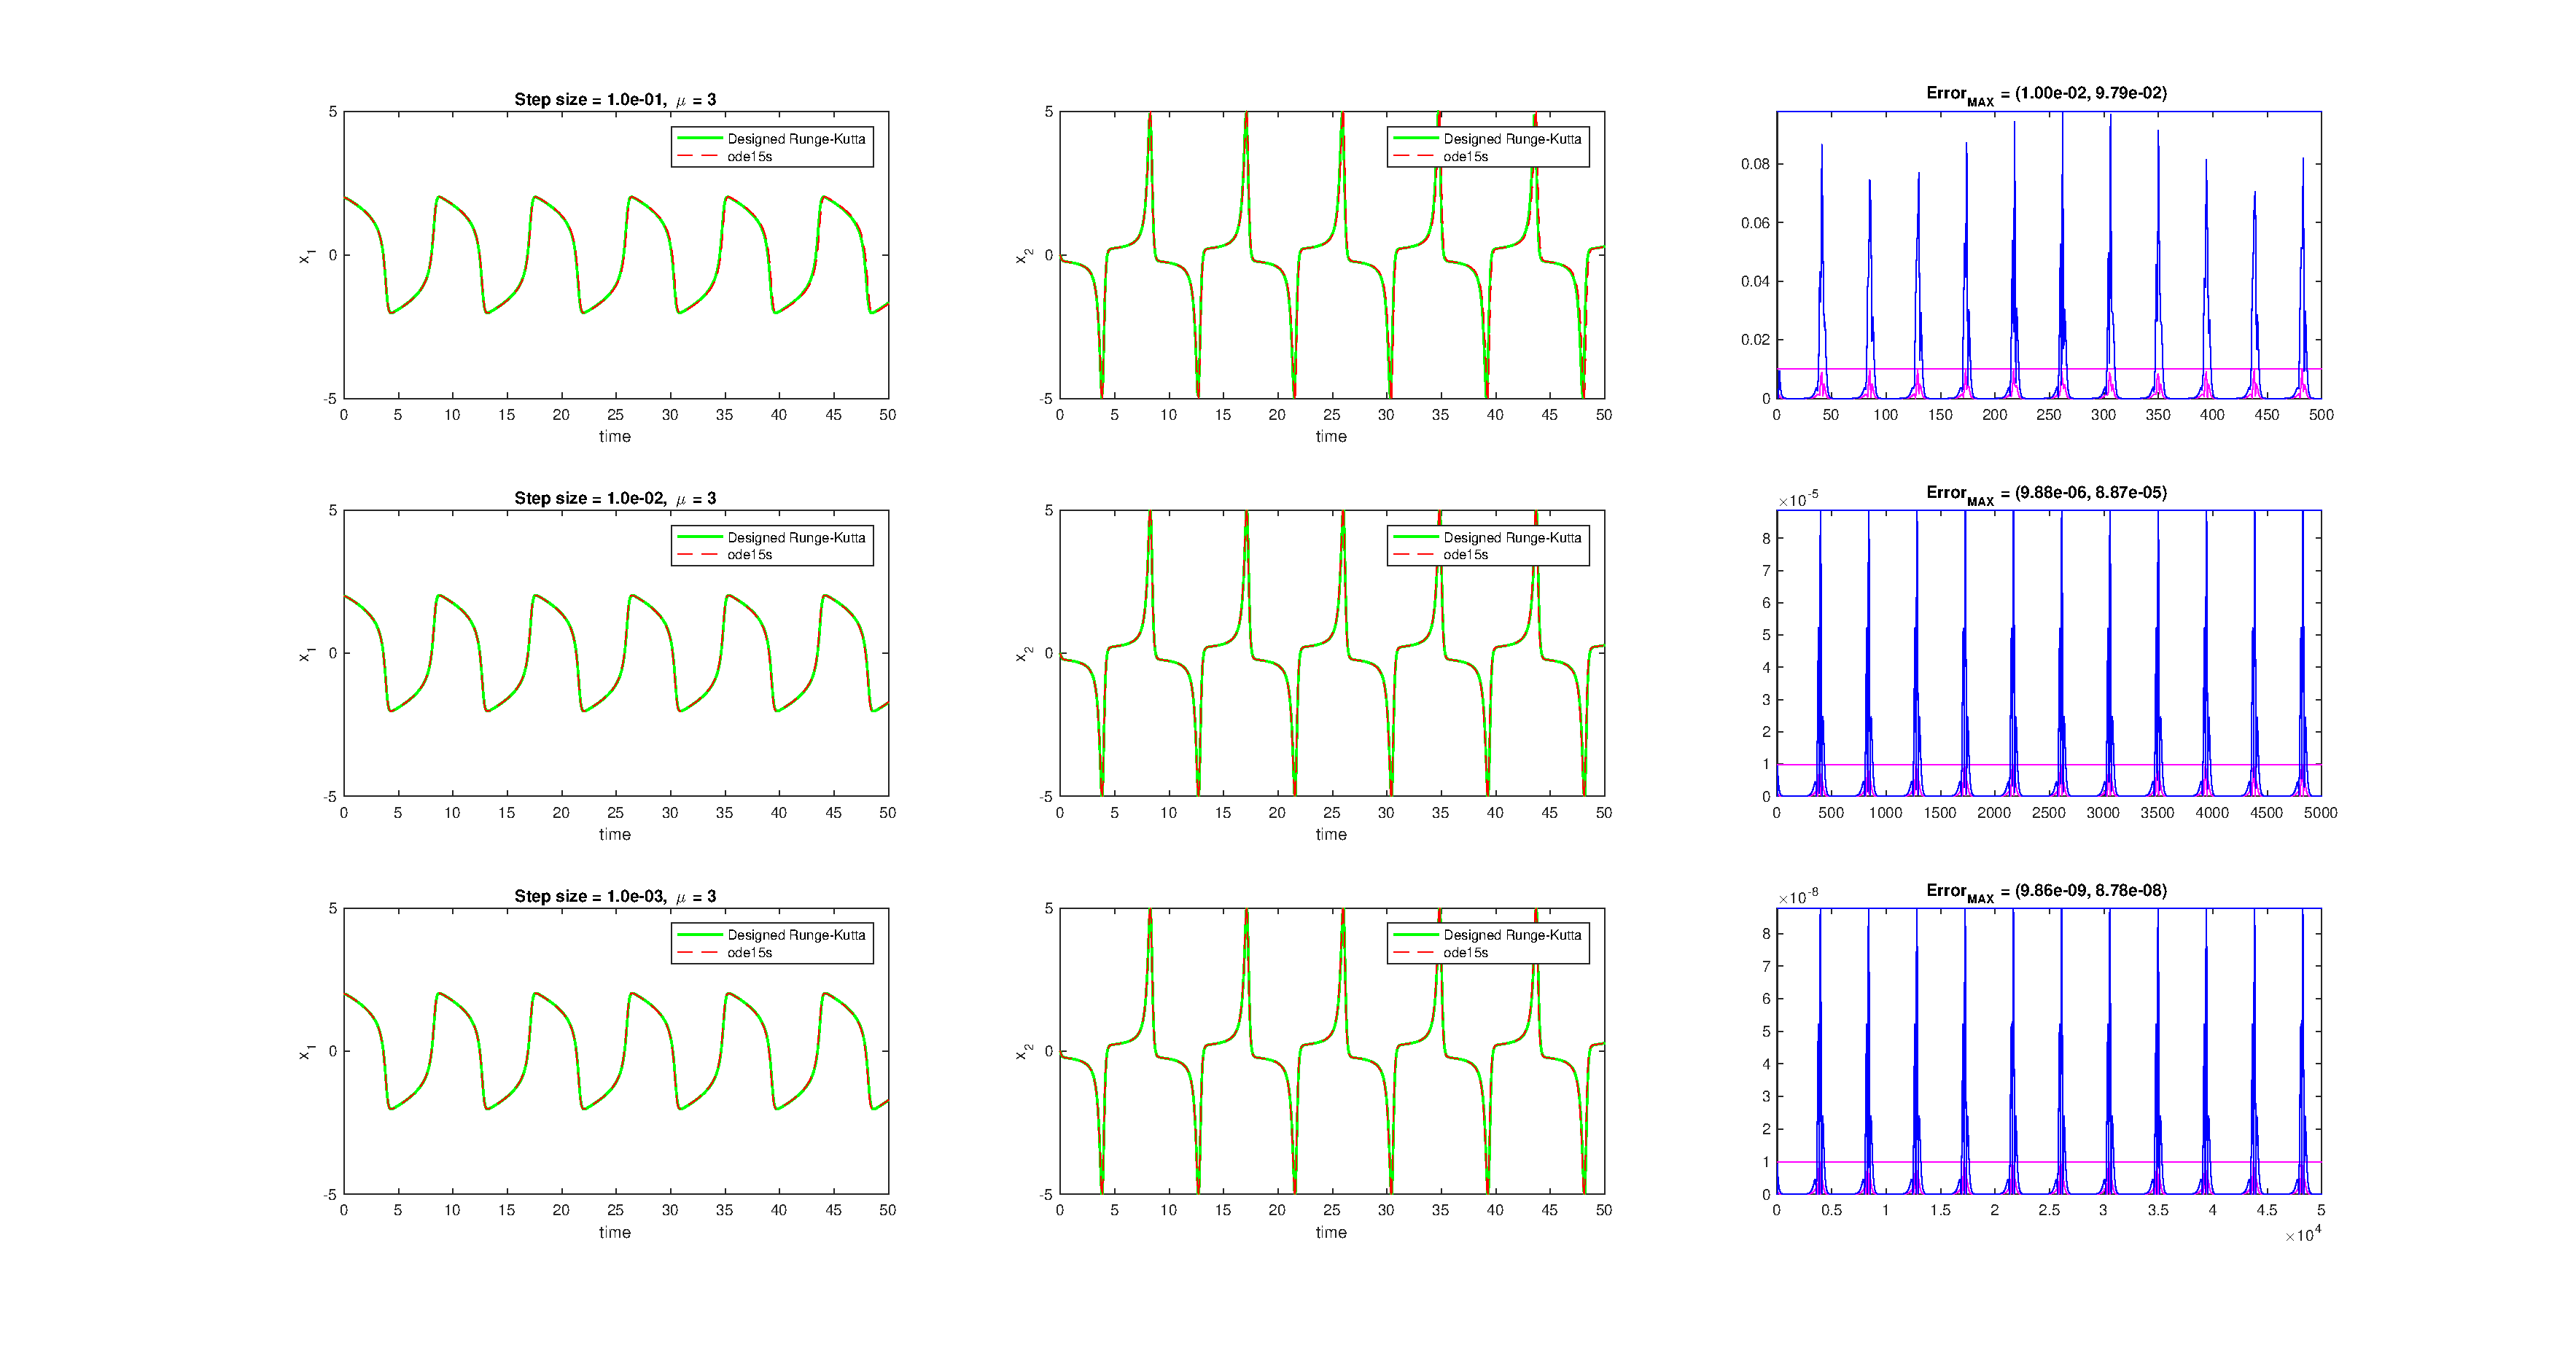
\includegraphics[width=\textwidth,trim={180 0 155 0},clip]{../Figures/ex3_vanderpol_ode15s}
    \caption{Comparison with \texttt{ode15s} on Van der Pol problem ($\mu=3$). Each row depicts different step size ($0.1$, $0.01$ and $0.001$) and the maximal error from ERK is shown in the plot title as well as on a reference line ($x_1$ - magenta, $x_2$ - blue).}
\end{figure}
